\documentclass[12pt]{unbthesis}
\usepackage[left=4cm, right=2.5cm, top=2.5cm, bottom=2.5cm]{geometry}
\usepackage{graphicx}
\usepackage{subfig}
\usepackage[subfigure]{tocloft} % no number for Vita in ToC
\usepackage{fancyhdr}
\usepackage[english]{babel}
\usepackage{csquotes}
\usepackage{footmisc}
\usepackage{algorithmic}
\usepackage{listings}
\usepackage{fancyvrb}
\usepackage[nottoc]{tocbibind}
\usepackage[hidelinks]{hyperref}
\usepackage{url}
\usepackage{dirtytalk}
\usepackage{listings}
\usepackage{xparse}
\usepackage{xcolor}
\usepackage{color}
\usepackage[]{algorithm2e}
\usepackage[utf8]{inputenc}


\definecolor{dkgreen}{rgb}{0,0.6,0}
\definecolor{gray}{rgb}{0.5,0.5,0.5}
\definecolor{mauve}{rgb}{0.58,0,0.82}
\definecolor{codegreen}{rgb}{0,0.6,0}
\definecolor{codegray}{rgb}{0.5,0.5,0.5}
\definecolor{codepurple}{rgb}{0.58,0,0.82}
\definecolor{backcolour}{rgb}{0.95,0.95,0.92}

\lstdefinestyle{CodeStyle}{
    backgroundcolor=\color{backcolour},   
    commentstyle=\color{codegreen},
    keywordstyle=\color{magenta},
    numberstyle=\tiny\color{codegray},
    stringstyle=\color{codepurple},
    basicstyle=\linespread{1}\ttfamily\footnotesize,
    breakatwhitespace=false,         
    breaklines=true,                 
    captionpos=b,                    
    keepspaces=true,                 
    numbers=left,                    
    numbersep=5pt,                  
    showspaces=false,                
    showstringspaces=false,
    showtabs=false,                  
    tabsize=2
}

\lstdefinestyle{CommandStyle}{
    backgroundcolor=\color{backcolour},   
    commentstyle=\color{codegreen},
    keywordstyle=\color{magenta},
    % numberstyle=\tiny\color{codegray},
    stringstyle=\color{codepurple},
    basicstyle=\ttfamily\scriptsize,
    breakatwhitespace=false,         
    breaklines=true,                 
    captionpos=b,                    
    keepspaces=true,                 
    % numbers=left,                    
    % numbersep=5pt,                  
    showspaces=false,                
    showstringspaces=false,
    showtabs=false,                  
    tabsize=2
}

% \lstset{style=CodeStyle}



\graphicspath{ {./Images/} }

\title{Behnam Fuzzer}
\author{Behnam Bojnordi Arbab}
\predegree{Previous Degrees (i.e. Degree, University, Year)\\
Bachelor of Computer Engineering, Ferdowsi University of Mashhad, 2015}
\degree{Master of Computer Science}
\gau{Computer Science}
\supervisor{Ali Ghorbani, Faculty of Computer Science}
\examboard{N/A}
\externalexam{N/A}
\date{Soon...!}
\copyrightyear{2020}
\setlength\parindent{0pt}
\newtheorem{theorem}{Theorem}[section]
\newtheorem{definition}{Definition}[section]
\newtheorem{lemma}{Lemma}[section]
\newtheorem{notation}{Notation}[section]

\NewDocumentCommand{\codeword}{v}{%
\texttt{\textcolor{blue}{#1}}%
}

\begin{document}
\unbtitlepage
\setcounter{secnumdepth}{3} \setcounter{tocdepth}{3}
\pagenumbering{roman} \setcounter{page}{1}

%%-------------Abstract-----------------
\doublespacing
\chapter*{Abstract}
\addcontentsline{toc}{chapter}{Abstract} 

Fuzz testing helps software security researchers investigate the existing vulnerabilities within programs in an automated fashion. AFL is a whitebox coverage-based fuzzer leveraging a genetic algorithm (GA) to search for vulnerabilities inside a program. The inputs to the program, which may affect the program's execution paths are considered as the individuals of GA, and the content of the files explain the genome. AFL investigates code coverages for the program's executions on each input, and the findings with new coverage information are selected for more testing. This technique guides the fuzzer to discover more regions of code. Waffle, is an AFL-based fuzzer searching for executions with higher resource usages, such as execution time. Waffle searches for files which not only discover new regions of code, but also require more resources to complete a run. Waffle modifies the instrumentation and fuzzing modules of AFL, with the intention of storing resource/time-consuming executions. To confirm the correctness of the modifications, the binaries are assessed, and the fuzzing procedure is monitored from a status screen. Finally, the performance of Waffle is compared to AFL-based fuzzers, and it is shown that Waffle discovers exhaustive executions effectively.
%% -----------Dedication----------------
\chapter*{Dedication}
\addcontentsline{toc}{chapter}{Dedication} Dedicated to knowledge.

\include{SideChapters/03-acknowledgments}

%%-----------Table of Contents------------------
\renewcommand{\contentsname}{Table of Contents}
\clearpage
\addcontentsline{toc}{chapter}{Table of Contents}
\tableofcontents{}
%%------------List of Tables----------------------
\clearpage
% \addcontentsline{toc}{chapter}{List of Tables}
\listoftables{}
%%------------List of Figures----------------------
\clearpage
% \addcontentsline{toc}{chapter}{List of Figures}
\listoffigures{}
\include{SideChapters/07-abbreviations}
%%-------------change single space to double space--------
\clearpage
\doublespacing
\pagenumbering{arabic}
\setcounter{page}{1}

\chapter{Introduction}
\label{chap:ch1}
\vspace{-30pt}

\section{Introduction}
\label{sec:intro}

% -T: Talk about software security testing and it's challenges
% -K: The needs which led to the usage of software
% -K: The daily tasks which are happening because of software
% -K: Explain the importance of keeping the software society safe

Our daily lives are tangled with the vast usage of software in many different aspects. Nowadays, most of the population in the modern world have a mobile phone in their hands, with hundreds or thousands of small to large software installed on their devices. Vehicles use software to monitor the sensors and react to different situations which help save and ease many lives. Instead of using mechanical tools and devices, the software can now do impossible calculations and suggest the most reliable solutions to different problems affecting our lives. Society communicates easier than before, and a world without the software would be unimaginable unless we choose less productivity and accept incomparable expenses. In a glance, huge loads of data are transmitted every second, and the services serve various customers using their technology. But the reliance of humanity on software establishes a weakness that hackers target. Thereby, security researchers and developers are responsible for stabilizing the field of software security.

% -T: Talk about the automation and fuzz testing
% -K: Explain how hard the software testing could happen
% -K: Explain the manual and automatic approaches for testing a software
% -K: Explain the benefit of using automated approaches

Software development has shown to be challenging, as unseen mistakes happen due to wrong approaches, or even worse, basically, because of possible human errors. The bugs may remain hidden for many years, and critical software must be investigated. The hackers are always looking for any vulnerability that helps them get past the protected areas. To investigate the bugs and prevent their existence, different phases of testing are applied before and after the accomplishment of products. One of the techniques for revealing bugs is to monitor the execution of a program and evaluate the correctness of the software's execution. A manual approach would be understanding source code and generated binaries and pointing out the present deficiencies and faults. This cumbersome task of reading the codes suggests the development of software security tools to speed up the testing. Fuzzer is an \textbf{automated software security testing} tool, which helps researchers find vulnerabilities, supported by the processing power of the computers.

\section{Summary of contributions}
\label{sec:1.2}

The fundamental goal of this thesis is to suggest a technique developed on AFL to identify the vulnerabilities related to excessive resource usages. The summary of our contributions follows:

% Improve fuzzing using llvm visitors.

\begin{itemize}
    \item For \textbf{instrumentations}, we have proposed a technique of instrumenting a program to log the usage of resources in runtime. To collect the information, we leverage the \textit{visitor} functions that LLVM project provides. We have empirically proved that the new instrumentation does not bring a noticeable overhead.
    
    \item We have changed the fuzzing procedure to consider the new instrumentations and enhance the generations of inputs with a higher number of executions of the specified visited instructions.
    
    \item We integerate the instrumentations and fuzzing procedure on top of AFL. Our experiments have shown an improvement in the code coverage of AFL. As the current version of our fuzz testing has introduced new bottlenecks, we may improve the code coverage more significantly. The source code is available on github \cite{wafl_git}.
\end{itemize}

\section{Thesis Organization}
\label{sec:1.3}

In Chapter 2, some of the related works in the area of fuzz testing are reviewed; software vulnerabilities and their occurrences are discussed, and a graphical representation of software is explained for understanding the execution of the program and unfolding the causes of vulnerabilities. Next, a classification of fuzzers and their usages are described. We wrap up the second chapter by introducing a fuzzer which is the base of our work. In Chapter 3, the proposed fuzzer is introduced. We explain how the solution is applied to a program with possible vulnerabilities. To wrap up the 3rd chapter, a sample program is tested, and the performance of the fuzz testing tool is analyzed. The performance of the implementations is evaluated in Chapter 4. A frontier benchmarking tool for fuzz testing is introduced, and the reports are presented afterward. We wrap up the thesis and conclude in Chapter 5. In addition, some future works are suggested for continuing this work.

%%-----------Chapters start-------------------------------------
%%-----------Chapter 1------------------------------------------
\chapter{Background}
\label{chap:ch2}
%\setcounter{secnumdepth}{3} \pagenumbering{arabic}
%\setcounter{page}{1} \pagestyle{myheadings}
%\markboth{}{}\markright{} \rhead{\thepage} \setcounter{page}{1}
%\pagestyle{myheadings} \pagenumbering{arabic} \rhead{\thepage}
%\setcounter{page}{1}

\section{Introduction}

The term \textbf{fuzzing} or \textbf{fuzz testing} was first introduced in late 80's. OWAPS defines it as a tool for \say{finding implementation bugs using malformed/semi-malformed data injection in an automated fashion}. \cite{owasp}

Since the growth of computer programs conquered all the globe, the profit of compromising the programs grew as well. 

\section{Literature Review} \label{sec:2.2}

Fuzzing searches for software vulnerabilities. "Vulnerability" has different definitions under various organizations and researches. For instance, \textit{International Organization for Standardization (ISO)} defines vulnerability as: \say{A weakness of an asset or group of assets that can be exploited by one or more threats, where an asset is anything that has value to the organization, its business operations and their continuity, including information resources that support the organization's mission.} \cite{iso27008} Yet, the definition needs more details for software. 

\subsection*{Software vulnerability}

According to the \textit{Open Web Application Security Project (OWASP)}: \say{A vulnerability is a hole or a weakness in the application, which can be a design flaw or an implementation bug, that allows attackers cause harm to the stakeholders of an application. Stakeholders include the application owner, application users, and other entities that rely on the application.} The existence of software vulnerabilities may be compromised and may become an attack target for hackers; this makes the software unreliable for its users. 

Various techniques are commonly used to identify weaknesses and vulnerabilities of a software. Techniques such as \textit{static analysis}, fuzzing, taint analysis and symbolic execution and etc. are of the most common techniques that can be used cooperatively for better results \cite{su2016vuldetection}. Static analysis evaluates the source code or binary for vulnerabilities, without executing the program.

\begin{algorithm}[!t]
  \KwIn{\textbf{$A, N$}}
  $i \leftarrow N$\;
  \SetKwRepeat{Do}{do}{while}
  \Do { $i >= 0$ } {
    $j \leftarrow 0$\;
    \Do {$j < i+1$} {
      \If{$A_j > A_{j+1}$} {
        $SWAP(A_j, A_{j+1})$\;
      }
      $j \leftarrow j+1$\;
    }
    $i \leftarrow i-1$\;
  }
  \caption{Pseudocode of bubblesort on array $A$ of size $N$}
  \label{algo:bubble}
\end{algorithm}

To investigate a program for bugs, a model that helps the research is \textbf{Control Flow Graph (CFG)}. CFG is a directed graph whose nodes are the basic blocks of the program, and its edges are the flow path of the execution between two consecutive basic blocks. For instance, the Figure \ref{fig:cfg} illustrates the CFG for \textit{bubblesort} algorithm (Algorithm \ref{algo:bubble}). The branches in CFG split after a \textit{conditional instruction} and a relevant \textit{jump instruction}.

\begin{wrapfigure}{L}{7cm}
  \includegraphics[width=6.5cm]{Chapter2/cfg.png}
  % \centering
  \caption{Control Flow Graph of bubblesort algorithm in Algorithm \ref{algo:bubble}}
  \label{fig:cfg}
\end{wrapfigure}

An execution processes a path (sequence) of instructions from an entry to any exit location of the program. For instance, consider Figure \ref{fig:cfg-heat} as a CFG illustrating the executed paths of 1000 trials of the program's execution. The numbers in the basic blocks indicate the number of times each basic block is visited. A path such as $A \rightarrow B \rightarrow E \rightarrow H \rightarrow I$ has been explored more than other execution paths. Basic block $D$ is visited occasionally and the edge $D \rightarrow I$ directly goes to the Exit, representing bugs in basic block $D$. These 1000 trials have discovered 9 seperable basic blocks, but it does not imply that there is no other basic blocks or edges revealed after more trials. Code coverage measures number of basic blocks which could be reached in an experiment of trials.

\begin{wrapfigure}{r}{6cm}
  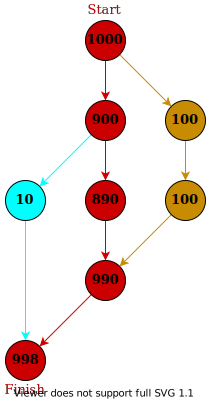
\includegraphics[width=5.5cm]{Chapter2/heatmap-cfg.png}
  \caption{CFG Heatmap \ref{algo:bubble}}
  \label{fig:cfg-heat}
\end{wrapfigure}

The vulnerabilities arise after target program executes with a triggering input. Miller introduced fuzz testing to examine the vulnerabilities of a collection of Unix utilities \cite{miller1990empirical}. The results showed that a random fuzzing on different versions of the utilities could discover bugs in 28\% of the targets. The automation in testing programs helps the researchers with validating the reliability of a program. The early fuzzers mimic a procedure of searching for the bugs by starting with \textit{identification} of the target program and its inputs. Next, the fuzzing loop initiates, and the program is run with fuzzed inputs as long as the fuzz testing is not terminated. Figure \ref{fig:fuzz_phases} depicts the fuzz testing procedure defined by Sutton et al. \cite{sutton2007fuzzing}. Based on the definitions, a standard fuzzer consists of:

\begin{itemize}
    \item Target identification
    \item Inputs identification
    \item Fuzzed data generation
    \item Execution of target with fuzzed data
    \item Exceptions monitoring
    \item Exploitability determination
\end{itemize}

\textbf{Target} is a software or a combination of executables and hardware \cite{song2019periscope}. A targeted software is any program that a machine can execute. 
Fuzzer needs to know the command for executing the target program and the inputs (arguments) of the program. \textbf{Inputs} are a set of environmental variables, file formats, and any other parameters that affect the execution. The initial seeds of the inputs can guide the fuzzer for finding more complex test cases, yet, it is not mandatory to provide seeds, and a fuzzer can generate valid inputs \textit{out of thin air} \cite{out_of_thin_air}. After the initial setup, the \textbf{fuzzing loop} begins iterating. In each iteration the fuzzer \textbf{executes} the target with the \textbf{provided test cases}. Fuzzer then looks for any exceptions returning from the executions and considers the executed input responsible for causing a \textbf{vulnerability}. The vulnerability can then be analyzed for \textbf{exploitability} in the last stage. An exploitable vulnerability can compromise the system and initiate an anomaly.

\begin{figure}[!b]
  \includegraphics[width=\textwidth]{Chapter2/FuzzingPhases.png}
  \centering
  \caption{Fuzzing phases. Inspired by the definition of Sutton et al. \cite{sutton2007fuzzing}}
  \label{fig:fuzz_phases}
\end{figure}

The categories for fuzzers with different \textbf{program awareness} and different \textbf{techniques for fuzzing} the inputs help the community find different applications of the fuzzers for discovering more vulnerabilities. For instance, a developer uses a whitebox fuzzer to assess the immunity of the program (source-code accessible) against malicious activities. On the other hand, an attacker may use a blackbox fuzzer to attack a remote program blindly. A researcher may use a coverage-based fuzzer to consider the execution paths as a variable to reach more regions of the code and detect more crashes; hence, another researcher may use a performance fuzzer to reveal the test cases causing performance issues. 

\subsection{Program awareness}

% It must be explained in more details that these colorful categories are not accurate. 

The \textit{colorful} representation of fuzzers depends on the amount of information collected from a symbolic/concrete execution. A blackbox fuzzer does not gather any information from the execution. In contrast, whitebox fuzzers have all the required access to the program's source code, and greybox fuzzing covers the gray area between the mentioned types.

% Executes a lot - Easily scaled - No program awareness
% Shallow bugs
% Blackbox fuzzer
\subsubsection{Blackbox fuzzing}

Blackbox fuzz testing is a general method of testing an application without struggling with the analysis of the program itself. The target of an analysis executes after calling the proper API's, and the errors are expected to occur in the procedure of trying various inputs. Blackbox fuzzing is an effective technique though its simplicity \cite{woo2013scheduling}.

The introduced fuzzer by Miller \cite{miller1990empirical} was of the very first naive blackbox fuzzers. It runs the fuzzing for different lengths of inputs for each target (of the total 88 Unix utilities) and expects a \textbf{crash}, \textbf{hang}, or a \textbf{succeed} after the execution of the program. Each input is then fuzzed with a random mutation to generate new test cases. One of the \textbf{downsides} of blackbox fuzzing is that the program may face branches with \textit{magic values}, constraining the variables to a specific set of values; for instance, as shown in Listing \ref{lst:magic}, the chance of satisfying the equation $\texttt{magic\_string=="M4G!C"}$ and taking the \texttt{succeed()} path is almost zero. In \cite{banks2006snooze} and \cite{gascon2015pulsar} a set of network protocols are fuzzed in a blackbox manner, but as the target is specified, the performance is enhanced drastically. Any application on the web may be considered a blackboxed program as well, so as \cite{doupe2012enemy} and \cite{duchene2012xss} have targeted web applications and found ways to attack some the websites, looking for different vulnerabilities, such as XSS.

\begin{lstlisting}[language=C++,style=CodeStyle,caption=Magic Value: \texttt{M4G!C} is a magic value,label={lst:magic}]
  string magic_string = random_string();
  if(magic_string == "M4G!C")
      return succeed();
  else
      return failed();
\end{lstlisting}

A blackbox fuzzer is unaware of the program's structure and cannot monitor it's execution. The \textbf{benefit} of using a blackbox fuzzer is the speed of test case generation; the genuine compiled target program is being tested and the fuzzer does not put an effort on processing the inputs and executions. In addition, a blackbox fuzzer is featured to target external programs by using the standard interfaces of those programs. For instance, IoTFuzzer \cite{chen2018iotfuzzer} is an Internet of Things (IOT) blackbox fuzzer, \say{which aims at finding memory corruption vulnerabilities in IoT devices without access to their firmware images.} 
In a recent research by Mansur et al. \cite{mansur2020detecting}, they introduce a blackbox fuzzing method for detecting bugs in Satisfiability Modulo Theories (SMT) problems. As a result, blackbox fuzzing suggests a general solution in diverse domains. On the other hand, one of \textbf{drawbacks} of using blackbox fuzzing is that it finds \textit{shallow} bugs. A shallow vulnerability is an error that appears in the early discovered basic blocks in the CFG of the program. The reason behind this disadvantage is that blackbox fuzzing is \textbf{blind} in understanding the execution, and cannot analyze the CFG.

% Whitebox fuzzers

\subsubsection{Whitebox fuzzing}
% !        Rewrite this  |
% TODO     Rewrite this  V
Whitebox fuzzing works with the source code of the target. In this technique, an \textbf{instrumentation} is applied before the compilation of the program. Whitebox fuzzing is not very practical in the industry as it is very expensive (time-consuming / resource-consuming) and faces many challenges. Symbolic execution \cite{king1976symbolic} is a common whitebox fuzzing strategy that analyzes the source code and runs the program symbolically; the variables and inputs are replaced by symbols that the solution specifies the domain of the content inputs. 

SAGE \cite{godefroid2012sage}, a whitebox fuzzer, was developed as an alternative to blackbox fuzzing to cover the lacks of blackbox fuzzers. With the benefit of having the source code and internal knowledge for fuzzing, a whitebox fuzzer can leverage symbolic constraints for symbolic analysis to solve the constraints (such as magic values) in the program \cite{cadar2011symbolic}. It can also use dynamic and concolic execution \cite{stephens2016driller} and use taint analysis to locate the regions of seed files influencing values used by program \cite{ganesh2009taint}. In addition, a whitebox fuzzer can find the grammar for parsing the input files without any prior knowledge \cite{godefroid2008grammar}.

\subsubsection{Greybox fuzzing}

Greybox fuzzing resides between whitebox and blackbox fuzzing, as it has partial knowledge (awareness) about the internals of the target program. A \textbf{concrete execution} of a program represents a reproducible procedure that is executed that can be monitored for its behavior detection.

\subsection{Generation of inputs}

A fuzzer can check the code coverage of the test cases to detect new inputs with new execution behavior. For a coverage-based fuzzing, the corpus of inputs extends as the fuzzer finds new execution-paths. A performance fuzzer guides the fuzz testing to detect more resource-exhaustive procedures, and the usage of specific resources is more preferable than the code coverage.

\subsubsection{Coverage-based fuzzing}

Coverage-based fuzzing is a technique for fuzz testing that instruments the target without analyzing the logic of the program. In a greybox and whitebox coverage-based fuzzing, the instrumentation detects the different paths of the executions \cite{liang2018fuzzing}. AFL instruments the program with only the coverage information (section \nameref{sec:2-afl}).

The instrumentation can collect execution's data such as data coverage, statement coverage, block coverage, decision coverage, and path coverage \cite{yang2009survey}. Bohme et al. \cite{bohme2017coverage} introduced a coverage-based greybox fuzzer that extends AFL and benefits from the Markov Chain model. The fuzzer calculates the \textbf{energy} of the inputs based on the potency of a path for the discovery of new paths.

In another article by Bohme et al. \cite{bohme2017directed}, they introduce their directed fuzzing by the idea of checking the code coverage for providing inputs that guide the program execution toward some targeted locations. Some of the applications of such a fuzzing approach are patch testing and crash reproduction, which has different use cases compared to a non-directed coverage-based fuzzers.

\subsubsection{Performance fuzzing}

The \textbf{types} of vulnerabilities that a fuzzer is involved with may be different from other fuzzers. For example, AFL looks for crashes or hangs by selecting and mutating the inputs, and at the same time, it considers the code coverage, size of the inputs, and each execution time of the target program. PerfFuzz \cite{lemieux2018perffuzz} is a greybox fuzzer based on AFL, which aims to generate inputs for executions with higher \textbf{execution time} while using most of the features of AFL in code exploration. PerfFuzz counts how many times each of the edges of the control flow graph (CFG) is executed. Using SlowFuzz \cite{petsios2017slowfuzz}, Petsios et al. lets the fuzzer use any execution features for detecting the worst-case scenarios (inputs) for the selected features. In another project based on AFL, Memlock \cite{wen2020memlock} investigates memory exhaustion by calculating the maximum runtime memory required during executions. A disadvantage in previous works in performance is that the development of the fuzzer for considering different instructions is cumbersome.

\vspace{1.5\baselineskip}


\section{LLVM} \label{sec:2-llvm}

% TODO: update llvm information in references
\say{The LLVM Project is a collection of modular and reusable compiler and toolchain technologies. The LLVM project has multiple components. The core of the project is itself called “LLVM.” This project contains all of the tools, libraries, and header files needed to process intermediate representations and converts them into object files. Tools include an assembler, disassembler, bitcode analyzer, and bitcode optimizer.} \cite{llvm,lattner2004llvm}

\vspace{\baselineskip}

LLVM can be used as a compiler framework, separated into "front-end" and "back-end." The front-end contains the lexers and parsers, and it accepts the source code to a program and returns the \textbf{intermediate representation (IR)} of the program. The back-end converts the IR into machine language.

\vspace{\baselineskip}

For instrumentation, we insert the logging instructions into each basic block of the program in the front-end. \textbf{Clang} is part of the LLVM toolchain for compiling C/C++ source code. By definition, \say{\textbf{clang} is a C, C++, and Objective-C compiler that encompasses preprocessing, parsing, optimization, code generation, assembly, and linking.}\cite{clang} We extend the phases of compilation so that we are injecting the instructions in compilation. 

\vspace{\baselineskip}

LLVM converts an \textbf{IR} of a program into machine language instructions. The structure of the LLVM project is shown in Figure \ref{fig:llvm}:

\begin{figure}[htpb]
    \includegraphics[width=\textwidth]{Chapter2/llvm.png}
    \centering
    \captionsetup{justification=centering}
    \caption{LLVM architecture: A front-end compiler generates the LLVM IR, and then it is converted into machine code \cite{omni_sci}}
    \label{fig:llvm}
\end{figure}

The instrumentation is applied before the IR generation, and the LLVM IR is fed into the LLVM compiler to generate the machine-specific instructions. As our instrumentation does not affect the LLVM IR compilation, we will not investigate the generated IR.

 
% Instrumentation
\subsection{Instrumentation and coverage measurements}
\label{instrumentation}

Waffle is based on AFL and we are extending the AFL's instrumentation in our work. The goal of using instrumentation for AFL is to differentiate code coverages. There are two techniques for instrumentation in AFL:

\begin{enumerate}
  \item \textit{$llvm\_mode$}: AFL takes the source code and an instrumentation recipe and generates the instrumented binary of the target program.
  \item \textit{$qemu\_mode$}: AFL leverages the QEMU mode to obtain instrumentation output for closed-source binaries. We don't use this mode in this thesis.
\end{enumerate}

In the LLVM recipe, we instantiate the bitmap and assign it to the shared memory for modifications. The remaining instructions for the recipe will be applied on the basic blocks in \textbf{AFLCoverage} module. This module takes effect in compilation of the program before the generation of IR. We can see some of the implementation of this \textbf{pass} in Listing \ref{lst:afl-llvm}:

\lstinputlisting[language=C++,style=CodeStyle,label={lst:afl-llvm},caption={AFLCoverage module}]{Codes/Chapter2/afl_llvm_pass.cpp}

The recipe for instrumentation fills out the coverage bitmap with the hash values of the paths executed. The instructions are as followed:

\begin{lstlisting}[language=C++,style=CodeStyle,label={lst:hash},caption={Select element and update in shared\_mem}]
  cur_location = <COMPILE_TIME_RANDOM>;
  shared_mem[cur_location ^ prev_location]++; 
  prev_location = cur_location >> 1;
\end{lstlisting}

AFL instruments by adding these instructions into basic blocks. First, a random value is assigned to \textit{curr\_location}. Next, it is XORed with the previous location's value, \textit{prev\_location}, and the resulting value is the location on \textit{shared\_mem}, the \textit{coverage bitmap}, which is incremented by one. The third and final instruction is reseting the \textit{prev\_location} to a new value.

\vspace{\baselineskip}

When AFL runs the instrumented program, every time an instrumented basic block is executed, a dedicated location of $shared\_mem$ in the bitmap is incremented. This algorithm recognizes the different paths that AFL runs through. For instance, in figure \ref{fig:instrumentation}, suppose that we have an instrumented program with the random values which is set in compile time. An execution that walks over basic blocks $1\rightarrow2\rightarrow5$ will increase the value of the corresponding locations by 1; for instance, an increment on $shared\_mem[14287 \oplus 23765]$ is applied for the transition of $1\rightarrow2$ and $shared\_mem[7143 \oplus 21689]$ for $2\rightarrow5$. We can see that the paths $1\rightarrow3\rightarrow4\rightarrow5$ and $1\rightarrow3\rightarrow4\rightarrow3\rightarrow4\rightarrow5$ (which contains a loop), set different locations on bitmap.


\begin{figure}[htpb]
    \includegraphics[width=\textwidth]{Chapter2/instrumentation.png}
    \centering
    \captionsetup{justification=centering}
    \caption{Example for instrumented basic blocks}
    \label{fig:instrumentation}
\end{figure}

AFL uses this coverage feature for discovering new inputs with new code coverages.

\subsubsection*{Visitor functions}

\say{Instruction visitors are used when you want to perform different actions for different kinds of instructions without having to use lots of casts and a big switch statement (in your code, that is). \cite{inst_visitor}} 

\lstinputlisting[language=C++,style=CodeStyle,label={lst:visitors},caption={Visitors example}]{Codes/Chapter2/visitor.cpp}

The specified range can be any two iterators, which can be a Module, Function, basic block, Instruction or any other range between two instruction addresses.

\section{AFL} \label{sec:2-afl}

Michal Zalewski initially developed American Fuzzy Lopper. He introduces this open-source project as \say{a security-oriented fuzzer that employs a novel type of compile-time instrumentation and genetic algorithms to automatically discover clean, interesting test inputs that trigger new internal states of the targeted binary. This substantially improves the functional coverage for the fuzzed code. The compact synthesized corpora produced by the tool help seed other, more labor- or resource-intensive testing regimes down the road.} \cite{zalewski2014american}

AFL is designed to perform \textbf{fast} and \textbf{reliable}, and at the same time, benefit from the \textbf{simplicity} and \textbf{chainability} of the fuzzer \cite{about_afl}:

\begin{itemize}
    \item \textbf{Speed:} Avoiding the time-consuming operations and increasing the number of executions over time.
    \item \textbf{Reliability:} AFL takes strategies that are program-agnostic, leveraging only the coverage metrics for more discoveries. This feature helps the fuzzer to perform consistent in finding the vulnerabilities in different programs.
    \item \textbf{Simplicity:} AFL provides different options, helping the users enhance the fuzz testing in a straightforward and meaningful way. 
    \item \textbf{Chainability:} AFL can test any binary which is executable, and is not constrained by the target software. A driver for the target program can connect the binary to the fuzzer.
\end{itemize}

\textit{afl-fuzz.c} has the instructions for fuzzing the target instrumented-program. The Algorithm \ref{algo:afl} illustrates a brief pseudocode of the execution of \textit{afl-fuzz}:

% main
%     initialize the fuzzer
%     while fuzzing is not terminated:
%         cull the queue of tests and update the bitmap
%         select the first entity of the queue, as E
%         fuzz(E)

% calibrate:
%     /* Calibrate a new test case. This is done when processing the input directory
%    to warn about flaky or otherwise problematic test cases early on; and when
%    new paths are discovered to detect variable behavior and so on. */

% trimming:
%     /* Trim all new test cases to save cycles when doing deterministic checks. The
%    trimmer uses power-of-two increments somewhere between 1/16 and 1/1024 of
%    file size, to keep the stage short and sweet. */

\begin{algorithm}
    % \DontPrintSemicolon % Some LaTeX compilers require you to use \dontprintsemicolon instead
    \KwIn{\textbf{$in\_dir$}, \textbf{$out\_dir$}, $instrumented$ \textbf{$Target$}}
    initialize fuzzer\;
    \While{fuzzing is not terminated} {
      cull queue and update bitmaps\;
      $Entry \leftarrow q.first\_entry()$\;
      $fuzz\_one(Entry)$\;
    }
    \caption{afl-fuzz}
    \label{algo:afl}
\end{algorithm}

After the environmental initializations, the fuzzing loop continues until receiving a termination signal. In every iteration of the loop, AFL first culls the corpus of the generated entries. This method assigns a \textbf{favor-factor} (Eq \ref{eq:afl_fav_fac}) to each queue\_entry and marks the \textbf{favorite entries}, as they execute faster and the size of the files are smaller than the rest of the corpus. AFL finds a favorable path for \say{having a minimal set of paths that trigger all the bits seen in the bitmap so far, and focus on fuzzing them at the expense of the rest.} \cite{afl_git} 
\begin{equation}
    fav\_factor = e.exec\_time \times e.length
    \label{eq:afl_fav_fac}
\end{equation}

An entry is selected after culling the queue. AFL evolves the input corpus by generating new entries out of the selected input entry - \texttt{fuzz\_one()}. 

\subsubsection*{fuzz\_one()}

% fuzz
%     calibrate the test case
%     trim the test cases (if needed)
%     calculate the performance score
%     bitflip
%     interesting values and dictionary usage
%     random havoc

\begin{algorithm}
    \KwIn{\textbf{$queue Entry$}}
    $T \leftarrow Entry.test\_case$\;
    $calibrate(T)$\;
    $trim(T)$\;
    $perf\_score \leftarrow calculate\_score(T)$\;
    \If{$deterministic\_mode$}{
      $deterministic\_stages(T)$\;
    }
    $MX \leftarrow calc\_stages(perf\_score, \mathcal{C})$\;
    \ForEach{element in $ (0, MX)$}{
      $random\_havoc(T)$\;
    }
    \caption{$fuzz\_one$: Fuzz one Entry}
    \label{algo:fuzzone}
\end{algorithm}

Fuzzing a single entry requires the calibration of the test-cases; calibration helps AFL in evaluating the stats of the current entry. This evaluation is stored in \texttt{perf\_score}, and the number of trials for generating new inputs from the \textbf{random\_havoc} stage is calculated using the \texttt{perf\_score}. AFL, as a coverage-based fuzzer, assigns higher performance score for the entries that are executed faster and have bigger bitmaps.

The evolutionary algorithms for generating new entries are applied in two stages: \textbf{deterministic} and \textbf{random\_havoc} stages. As shown in Algorithm \ref{algo:fuzzone}, AFL initially tries the basic, deterministic algorithms. These algorithms are executed for a specific number of times, in the same order, and once for each fuzzing trial. . Bit-flipping, byte-flipping, simple arithmetic operations, using known integers and values from dictionaries, are a sequence of mutations that AFL applies on an entry in \textbf{deterministic} stage. Each one of the above operations tweak a small portion of the fuzzed input, and does not modify the file in large portions - up to 32 bits changes in each tweak.

The \textbf{havoc} stage is a cycle of stacked random tweaks. AFL assesses the current entry to insert into the queue. Each mutation is selected randomly and with a higher \texttt{perf\_score}, this stage continues more fuzzing over the current entry. The \texttt{random\_havoc} stage consists techniques such as bit flips, overwriting with random and interesting integers, block deletion, block duplication, and (if supplied) assorted dictionary-related operations \cite{afl_userguide}. An abstract implementation of the \texttt{havoc\_stage} can be found in Appendix \ref{app:havoc}.

\subsubsection*{calculate\_score()}
\label{sub:calc_score}

This function calculates how much AFL desires to iterate in havoc stage, for the current entry. By default, AFL is interested in fuzzing an input with less execution-time, and simultaneously, showing more coverage, and it's generation depth is higher. The depth of a child entry is one more than the depth of it's parent. For more information, check the following abstraction of the function [Listing \ref{lst:calc_score}]: 

\lstinputlisting[language=C,style=CodeStyle,label={lst:calc_score},caption={An abstract implementation of calculate\_score()}]{Codes/Chapter2/calculate_score.c}

\subsubsection*{common\_fuzz\_stuff()}
The newly fuzzed (generated) inputs must pass \texttt{common\_fuzz\_stuff()} for validating and instantiating a \texttt{queue\_entry}. The validation checks the length of the fuzzed file, executes the program and keeps the exit-value of the execution. In the end, AFL calls \texttt{save\_if\_interesting()} to insert the entry into the queue, if it is interesting. The function \texttt{has\_new\_bits()} considers how interesting an entry is.

\lstinputlisting[language=C,style=CodeStyle,label={lst:common_stuff},caption={An abstract implementation of common\_fuzz\_stuff()}]{Codes/Chapter2/common_fuzz_stuff.c}

\subsubsection*{has\_new\_bits()}
AFL calls this function after each execution of the program, and the optimization of this code participates an important role.

\lstinputlisting[language=C,style=CodeStyle,label={lst:has_new_bits},caption={The implementation of has\_new\_bits()}]{Codes/Chapter2/has_new_bits.c}

\subsubsection*{Status screen}

The \textbf{status screen} is a UI for the status of the fuzzing procedure. As it is shown in Figure \ref{fig:status_screen}, there are multiple stats provided in real-time updates:
    
\begin{figure}[!b]
    \includegraphics[width=\textwidth]{Chapter2/afl_screen.png}
    \centering
    \caption{AFL status screen}
    \label{fig:status_screen}
\end{figure} 

\begin{enumerate}
    \item \textbf{Process timing}: This section tells about how long the fuzzing process is running.
    \item \textbf{Overall results}: A simplified information about the progress of AFL in finding paths, hangs, and crashes. 
    \item \textbf{Cycle progress}: As mentioned before, AFL takes one input and repeats mutating it for a while. This section shows the information about the current cycle that the fuzzer is working on.
    \item \textbf{Map coverage}: \say{The section provides some trivia about the coverage observed by the instrumentation embedded in the target binary. The first line in the box tells you how many branches we have already hit, in proportion to how much the bitmap can hold. The number on the left describes the current input; the one on the right is the entire input corpus's value. The other line deals with the variability in tuple hit counts seen in the binary. In essence, if every taken branch is always taken a fixed number of times for all the inputs we have tried, this will read "1.00". As we manage to trigger other hit counts for every branch, the needle will start to move toward "8.00" (every bit in the 8-bit map hit) but will probably never reach that extreme. 
    
    Together, the values can help compare the coverage of several different fuzzing jobs that rely on the same instrumented binary.
    }
    \item \textbf{Stage progress}: The information about the current mutation stage is briefly provided here.
    \item \textbf{Findings in depth}: The crashes and hangs and any other findings (here we have the other information about the coverage) are presented in this section.
    \item \textbf{Fuzzing strategy yields}: To illustrate more stats about the strategies used since the beginning of fuzzing, and for comparison of those strategies, AFL keeps track of how many paths were explored, in proportion to the number of executions attempted, for each of the fuzzing strategies.
    \item \textbf{Path geometry}: The information about the inputs and their depths, which says how many generations of different paths were produced in the process. For instance, we call the seeds we provided for fuzzing the "level 1" inputs. Next, a new set of inputs is generated as "level 2", the inputs derived from "level 2" are "level 3," and so on.
\end{enumerate}

\subsubsection*{Start Fuzzing}

AFL requires the instrumented binary for execution. To start the instrumentation, AFL uses \textit{afl-clang}, which is built with the coverage recipe included. The following command instruments the sample program \ref{lst:sample_vul}:

\begin{lstlisting}[language=bash,style=CommandStyle,caption=Instrument $sample\_vul$.c]
    afl-clang sample_vul.c -o sample_vul_i
\end{lstlisting}

Now AFL can run this program in \textit{afl-fuzz} with the coverage instrumentations.

\begin{lstlisting}[language=bash,style=CommandStyle,caption=Execute AFL]
  # afl-fuzz -i <in_dir> -o <out_dir> [options] -- /path/to/fuzzed/app [params]
  afl-fuzz -i in_dir -o out_dir -- ./sample_vul_i
\end{lstlisting}

The fuzzing continues until the fuzz testing is stopped using a termination signal. Pressing \textit{Ctrl+C} is a common command for this purpose. All of the recorded information are accessed through the output directory \textit{out\_dir}.

\section{Concluding remarks}

In this chapter we described some basics of our work, that inspired us and lets us implement the current version of our thesis, Waffle. The topics covered in this chapter are:

\begin{itemize}
    \item A brief description of the previous inspiring works for our fuzzer, as well as the stages of a fuzz testing procedure.
    \item We split different types of fuzzers into three categories, whitebox, blackbox, and greybox. These fuzzers have different access to the program resources and as a result, the fuzzing approaches were different.
    \item Code coverage and it's applications in fuzz testing is explained.
    \item We dig into the state-of-the-art fuzzer, AFL, and walked over it's stages that are important for our fuzzer.
    \item LLVM and it's applications in AFL, as well as the instrumentations done by AFL are described.
\end{itemize}

Altogether, we come up with a new approach for fuzzing, as we are aware of. These knowledge led us to introduce Waffle, which is explained in more details in the next chapters.

%%-----------Chapters start-------------------------------------
%%-----------Chapter 1------------------------------------------
\chapter{Proposed Fuzzer}
\label{chap:ch3}
%\setcounter{secnumdepth}{3} \pagenumbering{arabic}
%\setcounter{page}{1} \pagestyle{myheadings}
%\markboth{}{}\markright{} \rhead{\thepage} \setcounter{page}{1}
%\pagestyle{myheadings} \pagenumbering{arabic} \rhead{\thepage}
%\setcounter{page}{1}

% TODO: describe the 
% \section{Theoritical aspects}
% TODO: for instance, talking about how the Memfuzz is working
% TODO: talk about how our approach is going to be injected to the procedure of memfuzz

\section{Introduction}
In this chapter, we introduce \textbf{Waffle} in more details. Waffle is a tool capable of finding the vulnerabilities related to (theoretically) any resource exhaustion. The first section explains a motivating example leading to our proposed fuzzer. This fuzzer is based on AFL and extends its implementation. For monitoring the resources, we use compile-time instrumentation of the target program using LLVM's APIs; we take advantage of \textbf{visiting} APIs that let us keep track of any instructions defined for LLVM. As a result, the instructions related to any resource are counted, and this information is later used in the fuzzing stage.

AFL is the state-of-the-art in finding vulnerabilities and as it is amazing to be developed, the name of our fuzzer comes after \textit{WAAAFL}!

\vspace{\baselineskip}

In this chapter we are contributing the following topics:

\begin{itemize}
    \item An implementation of a fuzzer for finding the worst-case scenario in an algebraic problem.
    \item We use the \textbf{visitor} functions, which are not used in previous works, as we are aware of.
    \item A new instrumentation for collecting runtime information about resource usages. In Waffle, we focus on maximising the number of instructions.
    \item A new fuzz testing approach for collectively considering the former features of AFL, as well as the features we introduce in Waffle.
\end{itemize}

\section{Motivating example}

% TODO: talk about algorithmic problems, maybe
The intuition behind this thesis comes from the fact that all the programming competitions announce two main resources that are limited for the execution of the submitted program. This means that a program must be run without any compile-time or run-time errors and generate the correct output; and the whole execution is constrained with a specific time limit and memory limit. \cite{manzoor2008common} In some competitions, the judge system lets the competitors read each others' submitted program. If they can find a vulnerability in the program that is exploitable and causes any unexpected results, the hacker receives the score for their successful \textbf{hacking} attempt. \cite{wasik2018survey}

A fuzzer can automate the process of finding vulnerabilities; and targeting the algorithmic problems requires a resource-aware approach for investigating a larger range of problematic inputs.
\section{Instrumentation}
\label{sec:3-instr}

\subsubsection*{waffle-llvm-rt.o.c}

We initialize the instrumentation with setting up the shared memory for Waffle (Listing \ref{lst:llvm-rt}):

\lstinputlisting[language=C,style=CodeStyle,label={lst:llvm-rt},caption={LLVM instrumentation bootstrap}]{Codes/Chapter3/waffle-llvm-rt.o.c}

\texttt{\_\_wafl\_area\_ptr} is the region that is allocated for counting the instructions, and is later shared when the instrumented program is running in fuzz testing.

The size of the bitmap \texttt{\_\_wafl\_icnt\_ptr} is equal to $ICNT\_SIZE=2^{16}$; the size of the bitmaps are equal in both AFL and Waffle.

\subsubsection*{wafl-llvm-pass.so.cc}

Next, we inject our instrumentation into the program. As mentioned in the previous chapter, this stage requires the LLVM modules to analyze and insert the instructions. First, we define the \textbf{visitors}:

\begin{lstlisting}[language=C++,style=CodeStyle,label={lst:wfl-vis}]
struct CountAllVisitor : public InstVisitor<CountAllVisitor> {
  unsigned Count;
  CountAllVisitor() : Count(0) {}
  void visitMemCpyInst(MemCpyInst &I) { ++Count;}
};
\end{lstlisting}

We count the number of memory copies in an execution. The \texttt{CountAll\-Visitor} structure keeps track of the instructions that LLVM considers them as memory copies.

Now we can insert our instructions to the basicblocks:

\lstinputlisting[language=C,style=CodeStyle,label={lst:llvm-pass},caption={LLVM-mode instrumentation pass}]{Codes/Chapter3/mini-wafl-llvm-pass.so.cc}

In Line 7, we locate the shared bitmap. Lines 16 loads the pointer to the bitmap and configures the meta-data for storage \cite{nosanitize}.

Same as AFL, Waffle stores the counters in the \textbf{hashed value} of the path we explored (Listing \ref{lst:hash}). The usage of the coverage-guided hashed values, helps Waffle to collect coverage information, and at the same time, maximise the number of instructions in executions. The lines 21 to 23 loads the pointer to the appropriate location on the bitmap.

In each basicblock, the visitors look for the \textbf{copies}. In different executions, we noticed that the number of instructions increases so fast, and to control this number, we calculate its $\log$ (Lines 30-31):

\begin{equation}
  \label{eq:log}
  CNT = \log_{2}^{CAV} 
\end{equation}

Now that we have calculated \texttt{CNT}, we load the pointer on the bitmap and add \texttt{CNT} to the content of the pointer. Waffle stores the result of the addition in the same pointer. (Lines 36-39)

Waffle applies these instrumentation in the compile time, and when the program is run, the instructions have to add a number which is pregenerated, into the shared memory.

\subsubsection*{Applying the instrumentation}

To compile the target program with the adjusted instrumentation, we replace the C/C++ compilers (clang/clang++) with \textbf{\texttt{wafl-clang}}. \say{This program is a drop-in replacement for clang, similar in most respects to ../afl-gcc. It tries to figure out compilation mode, adds a bunch of flags, and then calls the real compiler.} \cite{clang-fast} Except refactoring the filenames and the name of the variables, we did not apply any other modifications on \texttt{wafl-clang.c}.

Same as \ref{lst:gcc-sample}, we can start instrumentation by the command below:

\begin{lstlisting}[language=bash,style=CommandStyle,label={lst:wafl-clang}]
  ./wafl-clang sample_vul.c -o sample_vul_instr
\end{lstlisting}

Notice that we can insert compilation flags, such as \texttt{-fsanitize=address}, to enhance the performance of Waffle.
% Can I add the IR here?
\section{Fuzzing}

% \lstinputlisting[language=C,style=CodeStyle,label={lst:llvm-rt},caption={LLVM instrumentation bootstrap}]{Codes/Chapter3/waffle-llvm-rt.o.c}

Waffle needs the instrumented binary from the previous section (\ref{sec:3-instr}) to start its fuzz testing loop. The input and output directories are specified for the fuzzer to work with. Next, Waffle takes one second for the timeout and considers no memory limit for each execution of the target program \cite{asan_note}. We also let the fuzzer work in deterministic mode, which we was discussed.

% According to the Algorithm \ref{}

% algo

% \input{Chapters/3-ProposedFuzzer/exploitability}
% \input{Chapters/3-ProposedFuzzer/shortcomings}
\newpage
\section{Concluding remarks}

This chapter introduced the development of Waffle. Waffle extends AFL in two parts:

\begin{enumerate}
    \item \textbf{Instrumentation}: \textbf{llvm\_mode} directory is responsible for the instrumentation in Waffle. As we explained in this chapter, \texttt{llvm\_mode/waffle-llvm-rt.o.c} contains the recipe for instrumenting the program in the compilation.
    
    AFL only keeps a coverage-bitmap, but in addition to the coverage-finding methodology, Waffle leverages the \textbf{visitor functions} in LLVM for assessing the more resource-exhaustive executions. Visitor functions count the targeted instructions, and Waffle saves the result in an extra \textit{shared\_memory}.

    Waffle counts the instructions in each basic-block, and reduces the counted values for saving into the memory. The size of the \textit{shared\_memory} has increased 4x in Waffle.

    \item \textbf{Fuzzing}: Waffle uses the coverage bitmap and the instruction-counter bitmap for emphasizing the more beneficial fuzzing entries. The main changes are in the procedures of the functions \texttt{calibrate\_case} and \texttt{calc\_score()}. Generally speaking, an interesting test-case runs faster, has more code coverage, and executes more instructions from a specified set of instructions.
\end{enumerate}

We also reviewed some of the modifications in the source code to Waffle's project. The project is located on github, in a public repository \cite{wafl_git}.
%%-----------Chapters start-------------------------------------
%%-----------Chapter 1------------------------------------------
\chapter{Simulation}
%\setcounter{secnumdepth}{3} \pagenumbering{arabic}
%\setcounter{page}{1} \pagestyle{myheadings}
%\markboth{}{}\markright{} \rhead{\thepage} \setcounter{page}{1}
%\pagestyle{myheadings} \pagenumbering{arabic} \rhead{\thepage}
%\setcounter{page}{1}
\section{Target program and instrumentation}
\section{Program inputs and setups}
\section{Generating fuzzed data}
\section{Program execution and monitoring}
\section{Report vulnerabilities}

% This is a subsection. This is \hfill a subsection.

%%-----------Chapters start-------------------------------------
%%-----------Chapter 1------------------------------------------
\chapter{Results and Evaluation}
%\setcounter{secnumdepth}{3} \pagenumbering{arabic}
%\setcounter{page}{1} \pagestyle{myheadings}
%\markboth{}{}\markright{} \rhead{\thepage} \setcounter{page}{1}
%\pagestyle{myheadings} \pagenumbering{arabic} \rhead{\thepage}
%\setcounter{page}{1}
\section{FuzzBench}
\section{results}
% This is a subsection. This is \hfill a subsection.

%%-----------Chapters start-------------------------------------
%%-----------Chapter 1------------------------------------------
\chapter{Conclusions and Future Work}
%\setcounter{secnumdepth}{3} \pagenumbering{arabic}
%\setcounter{page}{1} \pagestyle{myheadings}
%\markboth{}{}\markright{} \rhead{\thepage} \setcounter{page}{1}
%\pagestyle{myheadings} \pagenumbering{arabic} \rhead{\thepage}
%\setcounter{page}{1}
% \section{ A section}
% \subsection{A subsection}
% This is a subsection. This is \hfill a subsection.


% %%----------------Bibliography--------------------------------
\begin{thebibliography}{99}
\addcontentsline{toc}{chapter}{Bibliography}

\bibitem{k1} R.J. Drofnats, \emph{Proof of the Riemann
Hypothesis},  preprint, available at
\texttt{http://www.drofnats.com/riemann.ps}.

\bibitem{k2} P. Erd\H os, \emph{A selection of problems and
results in combinatorics}, Recent trends in combinatorics
(Matrahaza, 1995), Cambridge Univ. Press, Cambridge, 2001, pp. 1--6.

\bibitem{k3}
R.L. Graham, D.E. Knuth, and O. Patashnik, \emph{Concrete
mathematics}, Addison-Wesley, Reading, MA, 1989.

\bibitem{Knuth92} D.E. Knuth, \emph{Two notes on notation}, Amer.
Math. Monthly \textbf{99} (1992), 403--422.
\bibitem{Drofnats} R.J. Drofnats, \emph{Proof of the Riemann
Hypothesis},  preprint, available at
\texttt{http://www.drofnats.com/riemann.ps}.

\bibitem{Erdos01} P. Erd\H os, \emph{A selection of problems and
results in combinatorics}, Recent trends in combinatorics
(Matrahaza, 1995), Cambridge Univ. Press, Cambridge, 2001, pp. 1--6.

\bibitem{ConcreteMath}
R.L. Graham, D.E. Knuth, and O. Patashnik, \emph{Concrete
mathematics}, Addison-Wesley, Reading, MA, 1989.

\end{thebibliography}

% changes default name Bibliography to References
%\renewcommand{\bibname}{References}
\bibliographystyle{unsrt}
\bibliography{mybibliography}
%%---------------Appendices--------------------------------
\appendix
\chapter{Handling stack operations in Memlock}
\label{appendix:memlock}

\UseRawInputEncoding

The following code \ref{lst:memlock} is a shortend version of how memlock handles stack operations. In \textbf{line 6}, we can see that the \texttt{AFLCoverage} class is derived from a \texttt{ModulePass}, which runs a function pass over each function in the module. Using this pass, we can run over all instructions of IR. On \textbf{line 20} we define the pointer to the performance's array. In \textbf{lines 27} and \textbf{28}, we focus on each basic block; as a result, Memlock adds the instrumentations in each basic block. After loading the pointers that were defined earlier, on \textbf{line 53} Memlock defines \textbf{PerfTotalCounter}, for updating the corresponding pointer and in \textbf{line 54}, Memlock increments the counter of stack by one, if it is the first time we are visiting the current basic block. To figure out the type of instructions and find the \textit{return call instruction}, Memlock iterates over all instructions of the current basic block and compares the opcode of the instruction, with the opcode defined for return instruction (\textbf{line 58}). If the return instruction is found, the stack counter will be decreased by one.

Note that the following code is not the exact code and the source code can be found on Memlock project \cite{wen2020memlock}. Memlock handles the stack and heap operations in seperate files, doing different instrumentations for each of these two approaches.

\vspace{5mm}

\begin{lstlisting}[language=C++,style=CodeStyle,caption={Memlock C++ code for stack operations},label={lst:memlock}]
// required packages are included

using namespace llvm;

namespace {
  class AFLCoverage : public ModulePass {
    public:
      static char ID;
      AFLCoverage() : ModulePass(ID) { }

      bool runOnModule(Module &M) override;
      }
  };
}

bool AFLCoverage::runOnModule(Module &M) {
  LLVMContext &C = M.getContext();
  llvm::IRBuilder<> builder(context); 

  GlobalVariable *AFLPerfPtr =
      new GlobalVariable(M, PointerType::get(Int32Ty, 0), false,
                         GlobalValue::ExternalLinkage, 0, "__afl_perf_ptr");

  // To convert the range of EdgeID
  ConstantInt* PerfMask = ConstantInt::get(Int32Ty, PERF_SIZE-1);

  for (auto &F : M) {
    for (auto &BB : F) {
      BasicBlock::iterator IP = BB.getFirstInsertionPt();
      IRBuilder<> IRB(&(*IP));

      /* Load SHM pointer */
      LoadInst *MapPtr = IRB.CreateLoad(AFLMapPtr);
      MapPtr->setMetadata(M.getMDKindID("nosanitize"), MDNode::get(C, None));
      Value *MapPtrIdx =
          IRB.CreateGEP(MapPtr, EdgeId);

      /* Load the Performance Pointer */
      LoadInst *PerfPtr = IRB.CreateLoad(AFLPerfPtr);
      PerfPtr->setMetadata(M.getMDKindID("nosanitize"), MDNode::get(C, None));
      Value *PerfBranchPtr =
        IRB.CreateGEP(PerfPtr, IRB.CreateAnd(EdgeId, PerfMask));
  
      /* Increment performance counter for branch */
      LoadInst *PerfBranchCounter = IRB.CreateLoad(PerfBranchPtr);
      PerfBranchCounter->setMetadata(M.getMDKindID("nosanitize"), MDNode::get(C, None));
      Value *PerfBranchIncr = IRB.CreateAdd(PerfBranchCounter, ConstantInt::get(Int32Ty, 1));
      IRB.CreateStore(PerfBranchIncr, PerfBranchPtr)
          ->setMetadata(M.getMDKindID("nosanitize"), MDNode::get(C, None));
      
      /* Increment performance counter for total count  */
      LoadInst *PerfTotalCounter = IRB.CreateLoad(PerfPtr); // Index 0 of the perf map
      PerfTotalCounter->setMetadata(M.getMDKindID("nosanitize"), MDNode::get(C, None));
      Value *PerfTotalIncr = IRB.CreateAdd(PerfTotalCounter, ConstantInt::get(Int32Ty, 1));
      IRB.CreateStore(PerfTotalIncr, PerfPtr)
          ->setMetadata(M.getMDKindID("nosanitize"), MDNode::get(C, None));

      for(BasicBlock::iterator i = BB.begin(), i2 = BB.end(); i!=i2; i++) {
        IRBuilder<> MemFuzzBuilder(&(*i));

        if(Instruction *inst = dyn_cast<Instruction>(i)) {
          if(inst->getOpcode() == Instruction::Ret)
          {
            /* Subtract the memory usage of stack after return */ 
          }
        }
      }
    }
  }
  return true;
}
\end{lstlisting}

\include{SideChapters/09-glossary}
%%-------------Vita---------------------------------
\clearpage
\phantomsection  % correct link in PDF bookmarks.
\addtocontents{toc}{\cftpagenumbersoff{chapter}}  % omit page # in ToC
\addcontentsline{toc}{chapter}{Vita}
\chapter*{Vita}
\pagestyle{empty}
\thispagestyle{empty}
\singlespacing
Candidate's full name:\\
University attended (with dates and degrees obtained):\\
Publications:\\
Conference Presentations:

\end{document}
